\documentclass[11pt]{amsart}
\usepackage{geometry}                % See geometry.pdf to learn the layout options. There are lots.
\geometry{letterpaper}                   % ... or a4paper or a5paper or ... 
%\geometry{landscape}                % Activate for for rotated page geometry
%\usepackage[parfill]{parskip}    % Activate to begin paragraphs with an empty line rather than an indent
\usepackage{graphicx}
\usepackage{amssymb}
\usepackage{amsmath}
\usepackage{epstopdf}
\graphicspath{ {images/} }
\newtheorem{definition}{Definition}
\DeclareGraphicsRule{.tif}{png}{.png}{`convert #1 `dirname #1`/`basename #1 .tif`.png}

\title{Balancer: A protocol for multi-token automated market-making}
\author{Fernando Martinelli, Michael Zargham}
%\date{}                                           % Activate to display a given date or no date

\begin{document}
\maketitle
\section{Motivation}
%\subsection{}

As smart contracts gain traction and teams aim at leveraging real world usage, oracles become an ever more important component in the stack. Oracles make information from the outside world available for smart contracts. Arguably, one of the most important subset of that information, are price feeds. 

A wide range of projects in the blockchain space, such as MakerDao, depend on price feeds in order to function correctly. Current solutions to providing price feeds depend on external sources and usually require the payment of fees\footnote{https://docs.oraclize.it}. 

At BlockScience, we used our token engineering expertise and applied innovative invariant based modeling to achieve an on-chain price sensor for virtually any token pair. As for all our token engineering projects, the development was undertaken in 3 mains phases: 
\begin{enumerate}
    \item Requirements phase: what are the core requirements the system has to fulfill? In this first stage, we avoid being biased towards a specific solution. 
    \item Design phase: how can we achieve such requirements? A thorough functional analysis is performed, as well as the specification of the system core components
    \item Validation phase: is the system going to work as desired? After defining the requirements and the design, by means of extensive testing and simulation, we circle all the way back and prove that the initial requirements are met
\end{enumerate}

\section{Requirements}

\subsection{Introduction of Descriptive Model}

The Balancer is a token engineering project that applies BlockScience's innovative invariant based methods and modeling to achieve a much sought-after component in the blockchain space: a reliable on-chain price sensor. 

Even though our project is intended and designed to be blockchain-agnostic, we consider the Ethereum blockchain for practical reasons for this first instance. The balancer consists of a single smart contract that owns balances from a set of n different tokens. These tokens can be freely exchanged/traded by any external user interacting with the Ethereum blockchain.

All the $\frac{(n^2 - n)}{2}$ exchange rates between all the different n tokens are publicly available on-chain, at any time. These exchange rates are only dependent on the internal state of the Balancer smart contract, and they are automatically updated with each conducted trade. 

The main system requirement we set out with is that these contract-internal exchange rates closely follow the average external-market ones. Only then is an on-chain price-sensor useful and trustworthy for the blockchain community. 

A secondary, but equally important requirement, is that there should exist a measure of value of the tokens held by the contract that is strictly non-decreasing over time. That is, the contract owner that deposits the balances of n tokens into the Balancer smart contract can be certain that their value will never decrease. What's more, if a fee is charged for the usage of the contract by external users, this measure of value should be strictly increasing over time.

To achieve this, we seek to build a smart contract model that:

\begin{itemize}
    \item holds different balances of each of the $n$ tokens;
    \item has a simple-to-use, open and freely accessible external interface;
    \item possesses a rigorous mathematical dynamics that is proven to respect the requirement of being a reliable on-chain price sensor.
\end{itemize}

\subsection{Top-Level System Requirements}
The Balancer is not meant to be an instance of a contract but rather a class of contracts. Anyone is welcome to create their own instance of the Balancer, with their own choice of supported tokens. This leads us to the fact that the Balancer will always interact with two types of actors: 

\begin{itemize}
    \item any external blockchain users;
    \item the contract owner(s) - a strict subset of the above.
\end{itemize}

For simplicity, we always refer to external users as the users who are interacting with the Balancer contract but are not the contract owner(s).

Notice that in specific implementations, the owners of the contract may want to restrict which external users will be able to interact with the contract by enforcing a whitelist.

From a System Requirements standpoint, we can define two subsets of requirements: 

\begin{itemize}
    \item Internal Dynamics Requirements;
    \item Interface Requirements.
\end{itemize}

Figure 1 shows an overview of the Balancer System.

\begin{figure}
  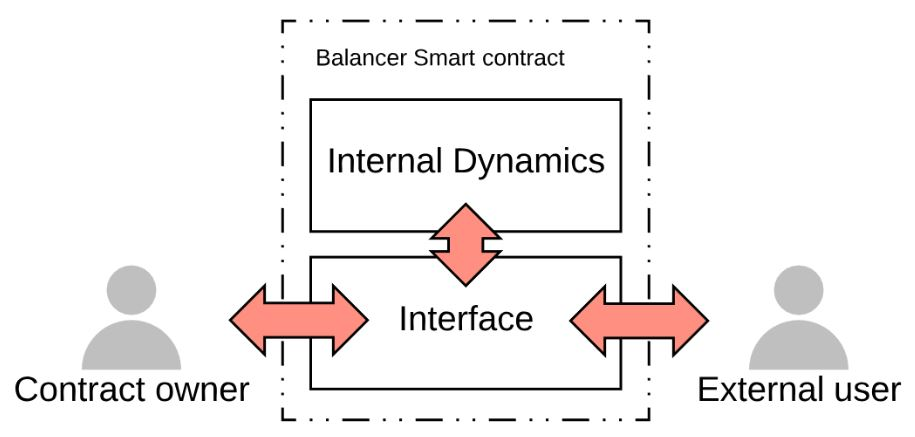
\includegraphics[]{overview}
  \caption{Top-level overview of the Balancer.}
  \label{fig:overview}
\end{figure}

\subsubsection{Internal Dynamics Requirements}

\begin{enumerate}
    \item \textit{Exchange rates are available for any pair of tokens held by the Balancer.} The internal dynamics should be such that, at all times, all $\frac{(n^2 - n)}{2}$ exchange rates are well defined and available upon external requests relayed by the contract interface. This may seem trivial but leads to special constraints that, for example, prevent the contract from running out of any given token, which would cause a division-by-zero error. 
    
    \item \textit{Exchange rates are updated as a function of trade volumes and internal balances.} The internal dynamics of the Balancer should be such that, if an external user intends to trade a lot of tokens A in return for tokens B, the Exchange Rate between those tokens is adequately updated such that the Balancer does not run out of tokens B. This Exchange Rate will depend on some variables like the current state of the contract (i.e. it's token balances) and the exact amount of tokens to be traded.
    
    \item \textit{The system shall provide resistance against the dumping of a token held in the contract whose value is approaching zero on external markets.} This is the other end of the curve discussed in the previous point. Instead of the contract running out of tokens, this requirement addresses protection against a contract being flooded with tokens that have no value on external markets. This may happen for example if a bug is found in the token contract, rendering it worthless.

\end{enumerate}

\subsubsection{Interface Requirements}

\begin{enumerate}    
    \item \textit{The Contract Owner is the only user that has the ability to withdraw funds.} The most crucial Interface Requirement is that no funds/tokens can be withdrawn by any External User except the Contract Owner.
    
    \item \textit{The External User action space shall be restricted to a bounded set of actions that preserve the 'Internal Dynamics' system requirements.} In order to achieve the main goal of being a reliable on-chain price sensor, the Balancer should have a well defined, rather restricted set of actions the External User is allowed to take. This is referred to as the External User action space. External users are restricted to trading any pair of tokens held by the contract, always one pair at a time.
    
    \item \textit{The Contract Owner shall maintain control over deposited funds, subject to a defined action space that preserves the 'Internal Dynamics' system requirements.} The Contract Owner is the responsible for deploying an instance of the Balancer and depositing tokens into it. They should, like the External User, have a well defined set of allowed actions. Since they are the owners of the tokens held by the Balancer, they should have full control over the funds they deposited to the Balancer up to the point that the internal dynamics of the contract is not invalidated.  
 
\end{enumerate}


\section{Design and Functional Specifications}

According to our system requirements, in order for our smart contract to be a reliable on-chain price sensor, it has to be at the same time a source of liquidity. The change in the amount of the individual balances of each of the $n$ tokens it holds is what will define the variation of the exchange rates sensed. This is modelled in a precise mathematical way, which provides the system with the required properties. 

Additionally, the more value the contract holds --i.e. the larger the balances of the $n$ different tokens supported--  the better and more dependable a price sensor it will be. The reason for this is that gaming it becomes more costly. 

At the same time, by holding large balances of the different supported tokens, the contract becomes a very useful source of liquidity for the Ethereum community. 

To ensure that there will be interest in making this liquidity available by deploying instances of our proposed smart contract, our design also fulfills the requirement that there should exist a measure of value of the tokens held by the contract that is strictly non-decreasing over time. From that perspective, the smart contract proposed can be seen as an auto balanced token index fund. However, instead of usual index funds that charge a fee, our proposed contract generates a fee, as we will see in the next sections.

Notice that our proposal is different from the Bonding Curve approach Simon de la Rouviere and others explore in Curation Markets\footnote{https://medium.com/@simondlr/tokens-2-0-curved-token-bonding-in-curation-markets-1764a2e0bee5} and Bancor uses in its protocol\footnote{https://storage.googleapis.com/website-bancor/2018/04/01ba8253-bancor\_protocol\_whitepaper\_en.pdf}. We do not need to create/mint a new token in order for our smart contract to work as intended.   

We now describe in detail our proposed specifications for the contract so as to achieve the requirements laid out above. 

\subsection{Mathematical framework}

Consider contract $C$ which contains $n$ different types of ERC20 tokens. Let's define the $n$-dimensional vector $Q^s \in \mathbb{R}_+^n$, representing the balances of each of the tokens supported for any given contract state $s$. As we'll prove in the following, the more tokens we have, the less slippage there is for a given trade. Since we'll probably have some key tokens that will be traded more often than others (think of ETH and DAI), it would be meaningful to have more value held by the contract in these tokens.  To do that, let's define the $n$-dimensional vector $w \in \mathbb{R}_+^n$, representing the value weights we'll assign to each of the tokens. We will initially assume $w$ constant, though the contract owner can change $w$ at any time for example if they want to add a new token to the contract or if they want to shift value between tokens.

Let's assume, for mathematical simplicity purposes, that the sum of all $n$ weights $w_{out}$ is equal to 1. If a token has twice as much weight than another one, this means that the contract will hold twice as much $value$ in that token --which does not mean twice as many tokens, of course.

Apart from the requirements discussed in the previous section, some further functional characteristics we are aiming to achieve with this contract are:

\begin{enumerate}
    \item No inherent preference or special treatment for one token over the other. They should be 100\% interchangeable;
    \item The ratio of token $out$'s balance $Q_{out}$ divided by it's weight $w_{out}$ and token $in$'s balance $Q_{in}$ divided by its weight $w_{in}$ at any time will be the spot exchange rate \footnote{Notice that to avoid any confusion we prefer to deal always with exchange rates as opposed to prices. Prices are the inverse of exchange rates: the higher the exchange rate of token $out$ in token $in$, the more tokens $out$ one gets with one token $in$} -- $SER^{out}_{in}$ -- between these two tokens held by the contract;
\begin{align*}
SER^{out}_{in} = \frac{\frac{Q_{out}}{w_{out}}}{\frac{Q_{in}}{w_{in}}} \end{align*}
    
    \item The share of value of each token in the contract is always proportional to its weight. That is, if one token gets more expensive relative to another, its amount decreases proportionally. 
\end{enumerate}

\subsection{Value function and contract methods}
Let's define value function $V^s$ which represents the value of the contract for any state $s$. This contract has essentially 3 methods, each having a different effect on $V$.

\begin{itemize}
    \item $trade$ (can be called by any external user): this function is meant for external users who want to trade any token j for tokens i. If, for simplicity's sake, we forego a trading fee charged to external users for trading, this method does not change $V$. $V$ is always invariant for trades within this contract. However, if we do consider a trading fee, then this function always slightly increases the value function $V$;
    \item $deposit$ (can only be called by the contract owner): this function allows the contract owner to deposit any tokens to the contract. This function can only increase the value function $V$;
    \item $withdraw$ (can only be called by the contract owner): this function allows the contract owner to withdraw any tokens from the contract. This function can only decrease the value function $V$.
    

\end{itemize}

We propose $V$ to be defined as
\begin{equation}
V = \prod_{k}(Q_k)^{w_k} 
\end{equation}

Let's also define the effective exchange rate an external user gets in any given trade as: 

\begin{equation}
EER^{out}_{in} = \frac{q_{out}}{q_{in}}
\end{equation}

where $q_{out}$ is the amount of tokens $out$ the user gets in return for sending an amount of $q_{in}$ tokens $in$. Notice that $EER^{out}_{in}$ depends on the amount $q_{in}$ of tokens $in$ the user sends, since there is slippage for any $q_{in}>0$. 

We'll now prove that the invariance of value function $V$ entails functional specification (2) as a corollary. By definition, the spot exchange rate is equal to the effective exchange rate when the amounts traded tend to 0. This limit can be calculated by taking the partial derivative of $Q_{out}$ in function of $Q_{in}$. Notice that we need to add a minus sign to the partial derivative since the amount of tokens $out$ the user gets in a trade is $subtracted$ from the contract:

\begin{equation}
SER^{out}_{in} = -\frac{\partial Q_{out}}{\partial Q_{in}}
\end{equation}

From eq. (1):

\begin{equation}
\begin{gathered}
(Q_{out})^{w_{out}} =  \frac{V}{\left(\prod_{k\neq out, k\neq outn}(Q_k)^{w_k}\right).(Q_{in})^{w_{in}}}\\
Q_{out} =  \left(\frac{V}{\left(\prod_{k\neq out, k\neq outn}(Q_k)^{w_k}\right).(Q_{in})^{w_{in}}}\right)^\frac{1}{w_{out}}
\end{gathered}
\end{equation}

Now we use eq. (4) to expand the derivative in eq. (3):

\begin{equation}
\begin{gathered}
SER^{out}_{in} = 
-\frac{\partial Q_{out}}{\partial Q_{in}} =
-\frac{\partial{\left(\left(\frac{V}{\left(\prod_{k\neq out, k\neq in}(Q_k)^{w_k}\right).(Q_{in})^{w_{in}}}\right)^\frac{1}{w_{out}}\right)}}{\partial Q_{in}}  =\\
=-\left(\frac{V}{\prod_{k\neq out, k\neq in}(Q_k)^{w_k}}\right)^\frac{1}{w_{out}}
.
\frac{\partial{\left(Q_{in}^{-\frac{w_{in}}{w_{out}}}\right)}}{\partial Q_{in}} =\\
=-\left(\frac{V}{\prod_{k\neq out, k\neq in}(Q_k)^{w_k}}\right)^\frac{1}{w_{out}}
.
-\frac{w_{in}}{w_{out}}.Q_{in}^{-\frac{w_{in}}{w_{out}}-1} =\\
=\left(\frac{V}{\prod_{k}(Q_k)^{w_k}}\right)^\frac{1}{w_{out}}
.Q_{in}^{\frac{w_{in}}{w_{out}}}.Q_{out}
.\frac{w_{in}}{w_{out}}.Q_{in}^{-\frac{w_{in}}{w_{out}}-1} = \frac{\frac{Q_{out}}{w_{out}}}{\frac{Q_{in}}{w_{in}}}
\end{gathered}
\end{equation}

which proves that our proposed invariant function $V$ fulfills functional specification (2).

\subsection{Trade function}

Once we have defined our invariant function $V$, calculating the trade function is easy, as it is a simple consequence of maintaining $V$ constant.

When a user sends tokens $in$ to get tokens $out$, all other token balances remain the same. Therefore, if we define $q_{in}$ and $q_{out}$ as the amount of tokens $in$ and $out$ exchanged, we can calculate the amount $q_{out}$ a users gets when sending $q_{in}$:

\begin{equation}
\begin{gathered}
(Q_{out}-q_{out})^{w_{out}}.(Q_{in}+q_{in})^{w_{in}} = Q_{out}^{w_{out}}.Q_{in}^{w_{in}} \\
Q_{out}-q_{out} = \frac{Q_{in}^{\frac{w_{in}}{w_{out}}}.Q_{out}}{(Q_{in}+q_{in})^{\frac{w_{in}}{w_{out}}}}\\
q_{out} = \left(1 - \left(\frac{Q_{in}}{Q_{in}+q_{in}}\right)^{\frac{w_{in}}{w_{out}}}\right).Q_{out}
\end{gathered}
\end{equation}

It is also very useful for traders to know how much they need to send of the input token $q_{in}$ to get a desired amount of output token $q_{out}$. We can calculate the amount $q_{in}$ as a function of $q_{out}$ similarly as follows:

\begin{equation}
\begin{gathered}
(Q_{out}-q_{out})^{w_{out}}.(Q_{in}+q_{in})^{w_{in}} = Q_{out}^{w_{out}}.Q_{in}^{w_{in}} \\
Q_{in}+q_{in} = \frac{Q_{out}^{\frac{w_{out}}{w_{in}}}.Q_{in}}{(Q_{out}-q_{out})^{\frac{w_{out}}{w_{in}}}}\\
q_{in} = \left(\left(\frac{Q_{out}}{Q_{out}-q_{out}}\right)^{\frac{w_{out}}{w_{in}}}-1\right).Q_{in}
\end{gathered}
\end{equation}

Notice that $q_{out}$ as defined by eq. (6) tends to $SER^{out}_{in}.q_{in}$ when $q_{in} << Q_{in}$, as expected. This can be proved by using L'Hopital's rule\footnote{https://en.wikipedia.org/wiki/L'Hopital's\_rule} but this proof is out of the scope of this paper.

For practical purposes, traders intending to use our contract for arbitrage will prefer to know what amount of tokens $in$ -- $q_{in}$ -- they will have to send to the contract to change the current spot exchange rate $SER^{out}_{in}$ to another desired one $SER^{out}_{in}'$. The desired spot exchange rate will usually be the external market exchange rate and, so long as the contract spot exchange rate differs from the external market's, any arbitrageur can profit by trading with the contract and bringing the contract exchange rate closer to the external market's. 

It's easy to prove that the highest profit possible by an arbitrargeur is when they bring the contract spot exchange rate exactly to the market's. This is the main reason why our design is successful in keeping track of the market prices, thus being a reliable on-chain price sensor.

It can be proved with a little math effort, which we consider out of this paper's scope, that the amount of tokens $in$ -- $q_{in}$ -- a user needs to trade against tokens $out$ so that the contract spot exchange rate changes from $SER^{out}_{in}$ to $SER^{out}_{in}'$ is:

\begin{equation}
\begin{gathered}
q_{in} = \left(\left(\frac{SER^{out}_{in}}{SER^{out}_{in}'}\right)^\frac{w_{out}}{w_{out}+w_{in}} - 1 \right).Q_{in}
\end{gathered}
\end{equation}

\subsection{Reference Token}

To prove that our mathematical framework also fulfills the requirement that "there should exist a measure of value of the tokens held by the contract that is strictly non-decreasing over time" let's define an imaginary token called Reference Token, or $RT$. The spot exchange rate of any token $out$ in the contract in terms of $RT$ tokens is defined as:

\begin{equation}
SER^{out}_{RT} = \frac{Q_{out}}{w_{out}}.\frac{1}{V}
\end{equation}

Notice that this definition of spot exchange rates for all tokens against the Reference Token is valid because it is fully consistent with all the $\frac{(n^2 - n)}{2}$ exchange rates of the tokens with respect to each other, as per the derivative calculated above:

\begin{equation}
SER^{out}_{in} = SER^{out}_{RT}.SER^{RT}_{j} = \frac{\frac{Q_{out}}{w_{out}}}{\frac{Q_{in}}{w_{in}}}
\end{equation}

By defining the exchange rates of all tokens against the $RT$ token as such, we can prove that the value in terms of $RT$ tokens of the total balance of any token $out$ -- $V_{out}$ -- is constant. This comes from the fact that the balance of each token decreases indirectly proportionally to its spot exchange rate in terms of $RT$:

\begin{equation}
V_{out} = \frac{Q_{out}}{SER^{out}_{RT}} = w_{out}.V 
\end{equation}

Notice also that the total value $V$ of the contract in  $RT$ tokens happens to be exactly $V$. This is no coincidence:

\begin{equation}
\sum_{k}V_k = \sum_{k}w_k.V = V.\sum_{k}w_k = V
\end{equation}

Reference Tokens can be seen as a weighted geometrical average amongst all tokens held by the contract. Their unit is $\prod_{k}(token\,k)^{w_k}$

\subsection{Auto-balanced index fund}

Eq. (10) summarizes the idea that this contract is an automatically balanced index fund in addition to being an on-chain price sensor -- which allows any blockchain user to trade the pairs of tokens it supports. By keeping function $V$ always invariant, it constantly exchanges tokens that become more valuable in return for those that become less valuable. Thus the amount of $value$ held by the contract in each token remains exactly the same at all times the contract is active. This value is equal to the total contract value times the weight of that corresponding token.

\subsubsection{Index fund value in USD}
We proved that the index fund has a constant value in terms of reference tokens $RT$. Therefore, one can calculate the variation of the total index fund value in terms of any other currency of interest -- for example USD -- by calculating the variation of value of one Reference Token relative to that other currency. 

Let's define $\Delta SER^{USD}_{RT}$ as the variation between two different contract states $s$ and $s'$ of the spot exchange rate of one reference token against USD:

\begin{equation}
\Delta SER^{USD}_{RT} = \frac{SER^{USD}_{RT}'}{SER^{USD}_{RT}}
\end{equation}

If $SER^{USD}_{RT}$ does not change between two different states, then the value of one Reference Token in USD is preserved, and $\Delta SER^{USD}_{RT} = 1$

It can be proved that the variation of value of one Reference Token in terms of any other currency, for example USD, can be calculated in terms of the variation of value of each token in the contract, weighted by their weights, as follows:

\begin{equation}
\Delta SER^{USD}_{RT} =\prod_{k}(\Delta SER^{USD}_{k})^{w_k}
\end{equation}

To help visualize the practical meaning of this equation, imagine a contract with only 2 different tokens, each with weight $0.5$. Suppose that:

\begin{itemize}
    \item token 1 doubled its exchange rate in USD -- i.e, a token 1 is now worth twice as much USD as before;
    \item token 2 trippled its exchange rate in USD -- i.e, a token 2 is now worth three times as much USD as before.
\end{itemize}

Then the total value of the contract in USD would increase by a factor of:

\begin{equation*}
\Delta SER^{USD}_{RT} =\prod_{k}(\Delta SER^{USD}_{k})^{w_k} = 2^{0.5} . 3^{0.5} = 2,449...
\end{equation*}

\subsection{Fees}

In order to incentivize the creation of instances of this auto-balanced index fund smart contract, we propose that the contract charge traders a fee $f$ which is a percentage of the tokens they send in for trading. This is industry standard for any exchange, centralized or not. Traders are used to paying a trading fee, especially considering that external users trading with our contract are comparable to liquidity "takers" on conventional exchanges -- as they execute a trade on the spot exchange rate as opposed to creating an order that may be fulfilled in the future (AKA liquidity "makers".

To account for this fee in our mathematical framework, instead of using the amount of tokens $q_{in}$ sent by a user trading tokens $in$ for tokens $out$, we simply calculate the amount of tokens $out$ to be received by using $q_{in}'$ instead of the actual amount sent $q_{in}$, where $q_{in}' = q_{in}.(1-f)$. The fee $q_{in}. f$ can be considered revenue for the contract owner, as it will increase the value function $V$ of the contract.

\section{Validation}

** Here goes all the testing results proving that under different conditions and external users with different behaviors, the contract sensed price converges to the external market price. **

\subsection{Example}

Let's say we have a contract that has three tokens: DAI, ZRX and WETH.

We expect WETH to be a primary exchange token -- that is, pairs containing it will be more often traded -- so we want to have more value stored in it for traders to suffer the least slippage possible. We define then $w_{DAI} = 0.25$, $w_{ZRX} = 0.25$ and $w_{WETH} = 0.5$. Considering DAI, ZRX and WETH prices in USD as respectively 1, 2 and 650, a possible initial balance of the contract could be $Q = [650, 325, 2]$. In this case, the reference token RT would have unit $DAI^{0.25}.ZRX^{0.25}.WETH^{0.5}$. The exchange rates of DAI, ZRX and WETH in RT would be respectively 0.666,	1.332 and 433.0.

\end{document}  